
\subsection{Algorithms}
\label{sec:algorithms}
%We performed protein function prediction using three networks-based methods---\genemania, and \SS
%~\begin{NoHyper}\cite{murali-katze-network-based-prediction-hiv-ploscb-2011}\end{NoHyper}---%
%that propagate evidence across the entire network from genes annotated with a GO term (positives) to genes not known to have the function (unknowns). 
%We compared with a baseline that we called Local+ in which each protein's prediction score for a GO term is the weighted average of the scores of its neighbors. This is akin to how predictions are normally made using BLAST.


\paragraph{\sinksource.} 
%The \sinksource algorithm can be understood via an analogy to electrical circuits where positive nodes are connected to a voltage of one Volt 1V, negative nodes to a ground (0V), and each edge weight is treated as a conductance. The amount of voltage on each unknown is the final prediction score and can be computed by minimizing the weighted difference between score of every pair of neighbors. 
Given a weighted, undirected network $G = (V, E)$, %with $n = |V|$ and $m = |E|$ as a $n \times n$ square matrix $W$, 
where $w_{uv}$ indicates the weight of the edge $(u,v)\in E$,
and $V$ partitioned into three subsets $V^+$, $V^0$, and $V^-$ for positive, unknown and negative examples respectively, the goal of \sinksource is to compute a score $s$ between $0$ and $1$ for each node $u$ in $V^0$ to assess whether $u$ should be a member of $V^+$ or $V^-$. 
The scores of nodes in $V^+$ and $V^-$ are fixed to 1 and 0 respectively.
%By fixing the score of nodes in $V^+$ and $V^-$ to 1 and 0 respectively, \sinksource computes scores for the unknown nodes in $V^0$ by minimizing the weighted difference of each node's score with that of its neighbors in $G$ ($N(u)$). Specifically, 
\sinksource then computes a score for each unknown node $u$ by minimizing the weighted difference of each node's score with that of its neighbors in $G$ (denoted by $N(u)$). Specifically, it requires that $s$ minimize the function
%Specifically, we set $s(u) = 1$ for each node $u$ in $V^+$, $s(u) = 0$ for every node $u$ in $V^{-}$, and required that the $s$ minimize the function

\begin{equation}
    S(G,s) = \sum_{\mathclap{(u,v)\in{}E}} w_{uv}\left(s(u) - s(v)\right)^2
    %S(W,\vec{s}) = \sum_{u,v = 1}^{n} W_{uv}(s_u - s_v)^2
\end{equation}
The function $S(G,s)$ is minimized when, for each node $u$ in $V^0$, 
\begin{equation}
\label{eq:sinksource-minimized}
    s(u) = \frac{\sum\limits_{\mathclap{v \in N(u)}}\hspace{2.5pt} w_{uv} s(v)}{d(u)}
    %s_i = \frac{\sum\limits_{j = 1}^{n} W_{ij} s_i}{\sum\limits_{j = 1}^{n} W_{ij}}
\end{equation}
where $d(u) = \sum\limits_{\mathclap{v \in N(u)}} w_{uv}$ is the weighted degree of $u$.
Because positive and negative examples have a score fixed at 1 and 0 respectively, we can separate \cref{eq:sinksource-minimized} into two parts: one corresponding to contributions from neighbors in $V^0$ and the second to a constant contribution from neighbors in $V^+$ as follows
\begin{equation}
%\label{eq:sinksource-minimized-split}
    s(u) = \frac{\sum\limits_{v \in N^0(u)} w_{uv} s(v)}{d(u)} + f(u)
\end{equation}
where $f(u) = \frac{\sum\limits_{v \in N^+(u)} w_{uv} }{d(u)}$
and $N^0$, and $N^+$ are neighbors in $V^0$ and $V^+$ respectively.
Note that negative examples are fixed at $0$ and therefore do not contribute to the score.
Let $\vec{s}$ denote the vector of scores for the nodes in $V^0$. 
Let $P$ denote a square matrix where $P_{uv} = w_{uv} / d_u$ for every $(u,v) \in V^{0}$.
We can compute $\vec{s}$ by solving the following linear system
\begin{equation}
\label{eq:sinksource-matrix-iteration}
    \vec{s} = P\vec{s} + \vec{f}
\end{equation}
where $\vec{f}$ is a fixed vector containing contributions from $V^+$ and $\vec{s}$ starts at all $0$s.
We compute $\vec{s}$ by repeatedly applying \cref{eq:sinksource-matrix-iteration}. % which we refer to as ``power iteration''. 
This process is known to converge~\cite{zhu-lafferty-semi-supervised-learning-icml-2003}, resulting in a value of $\vec{s} = (I - P)^{-1} \vec{f}$.
%\jeff{scipy has a bug where I am unable to solve it directly for large sparse matrices}
\jeff{We solve this system by ...}


\paragraph{\genemania.}
Given a composite network $W$ and a label vector $\vec{y}$ where $y_u$ represents the prior evidence for gene $u$ having a function of interest, the GRF algorithm assigns a discriminant score $s_u$ between $-1$ and $1$ to each gene $u$ in the network, which we can threshold to classify the genes.
In particular, $y_u = {-1,k,+1}$ where given negative ($n^-$) and positive ($n^+$) examples are assigned -1 and +1 respectively, and $k = \frac{n^+ - n^-}{n^+ + n^-}$, the mean of the labels of the labelled nodes, is assigned to the unknown nodes.
The final vector containing the scores for each node is obtained by solving the optimization problem:

\begin{equation}
    \vec{s} = \min \limits_{\vec{s}} \bigg( \sum_{u=1}^{n} (s_u - y_u)^2 + \sum_{u,v=1}^{n} W_{uv}(s_u - s_v)^2 \bigg)
    %\fvec = \min\limits_{\fvec} \sum\limits_{i=1}^{n} (f_i - y_i)^2 + \sum_{i,j=1}^{n} W_{ij}(f_i - f_j)^2
\end{equation}

To solve for $\vec{s}$, we only need to solve a linear system of equations $M\vec{s} = \vec{y}$, where $M = (I + L)$, $L = D - P$ is the Laplacian of the graph, $D$ is a diagonal matrix with $D_{uu} = \sum_v W_{uv}$ and $P = D^{-1/2} W D^{-1/2}$.

To solve this linear system, we utilized the conjugate gradient (CG) solver implemented in the SciPy (v1.1.0) Python package and used the default tolerance cutoff of \e{-5}. 

\paragraph{\birgrank.}
%\birgrank (BI-Relational Graph page RANK) constructs a bi-relational graph with a given \FLN and a GO hierarchy, where genes are connected by an edge to GO terms for which they have an annotation, 
%and then directly applies PageRank to diffuse the annotation information across the two-layer network. 
\birgrank differs from \sinksource and \genemania in a few major ways. 
First, it directly incorporates the GO hierarchy into the diffusion process.
Second, \birgrank{}'s propagation is done on a gene-by-gene basis, meaning it makes all function predictions for a single gene simultaneously. Third, it does not incorporate negative examples.
%In their evaluations, Jiang \etal demonstrated significant improvements of \birgrank over many other network propagation methods such as \genemania and others which incorporate the GO hierarchy in some way such as clusDCA~\cite{wang-pang-clusdca-exploit_ontol_graph-bioinfo-2015}. %~\cite{wang15_exploit_ontol_graph_predic_spars}.%.  
%We included \birgrank here in our evaluations in the hopes that we would see similar improvements in prediction performance.
\jeff{We opted to compare with the simpler \birgrank as it was much simpler and faster than AptRank, yet showed similar improvements in many of their evaluations.}
%Here we 

For every gene - GO term annotation pair $g$-$t$, there is a corresponding $g$-$t$ edge in the annotation matrix $R$ with a weight of one.
\birgrank has various parameters to control the propagation flow and direction between $G$ and $H$. $\mu$ controls the proportion of flow within $G$ vs.\ flow to $H$, $\theta$ controls the amount of restart from a given gene vs.\ the functions annotated to it, and $\lambda$ controls the direction of flow in the hierarchy with $H^* = \lambda H + (1 - \lambda)H^T$.

To compute the prediction scores, \birgrank solves the system of linear equations
\newcommand{\overbar}[1]{\mkern 5.5mu\overline{\mkern-5.5mu#1\mkern-5.5mu}\mkern 5.5mu}

\begin{equation}
\bigg( \hspace{-2pt}
\begin{bmatrix} I_m & 0 \\ 0   & I_n \end{bmatrix} - \alpha 
\overbar{ \begin{bmatrix} \mu G & 0 \\ (1-\mu)R^T & H^* \end{bmatrix} }
\hspace{-2pt} \bigg)
\begin{bmatrix} X_G \\ X_H \end{bmatrix}
 = (1-\alpha)
 \begin{bmatrix} \theta I_m \\ (1-\theta)R^T \end{bmatrix}
\end{equation}

where the bar over the block matrix indicates the the whole matrix is column normalized. 
The lower block of the solution, $X_H$, contains the function prediction scores for each node and has the same dimensions as $R^T$.

%- \mu: controls the proportion of flow within $G$ 
%- $H^* = \lambda H + (1-\lambda)H^T$
%  - $\lambda$: controls direction of heirarchy
%- \theta: controls the weighted sources between the proteins and functional annotations

% annotations
In the original work by Jiang \etal, they built the annotation matrix $R$ using only direct annotations, meaning they did not propagate annotations up the GO hierarchy according to the annotation rule. As we are evaluating on a term-by-term basis, we opted to include all propagated annotations in $R$ to allow \birgrank to utilize those connections when making predictions.

In the original MATLAB implementation of \birgrank, the authors solved for all nodes in $X_G$ and $X_H$ directly, making predictions for all nodes simultaneously. 
%Unfortunately 
%As \birgrank propagates scores from genes in $G$ to the GO term nodes, 
We found we were able to greatly reduce the runtime of \birgrank by solving only for the nodes for which we are validating in a given evaluation, rather than all nodes. Additionally, we computed the RWR scores using power iteration until the maximum difference of node scores between iterations $i$ and $i-1$ was $\leq$ \e{-4}. 




We implemented each of the above algorithms in Python using SciPy (v1.1.0) and NumPy (v1.15). In cases where the algorithm was already implemented in MATLAB (\genemania, \birgrank), we essentially performed a line-by-line translation of the MATLAB commands to SciPy sparse matrix commands. We ensured the correctness of our implementations by comparing our output values to those output by the MATLAB implementation. They matched exactly. 

\subsection{Speed-up}
\label{sec:speed-up}

Currently, all of these methods use either power iteration or other linear system solvers such as conjugate gradient. 
Power iteration, and typically other solvers, rely on a stopping criteria to know when the scores have converged "enough". 
The algorithms continue to iterate until the maximum difference of node scores from iteration $i-1$ to $i$ is $\leq \epsilon$, where epsilon is a pre-defined parameter typically around \e{-4} \jeff{cite}. 
In our use of \sinksource, we found that for most GO terms, in order to reach a reasonable value of $\epsilon$, hundreds to thousands of iterations were required~\jeff{Need to add data supporting that claim}. 
We questioned which values of $\epsilon$ were appropriate? Is there a better stopping criteria than $\epsilon$?


%In our efforts to find a way to speed-up \sinksource, we discovered that a recent method for efficiently computing the top-k nodes with the highest RWR scores from a query called Squeeze~ \cite{zhang-han-ripple-fast-topk-rwr-kdd-2015} has an update equation (for power iteration) very similar to that of \sinksource (see supp. for comparison).
A recent method for efficiently computing the top-k nodes with the highest RWR scores from a query node, called Squeeze, works by computing a lower- and upper-bound for each node after each step of power iteration. Squeeze continues to iterate until the lower-bounds of the top-k node scores are all higher than the upper-bounds of the rest of the nodes in the graph, thus ensuring the top-k nodes have been found.


Every iteration takes each node closer and closer to its final score and at a given iteration $i$, the current score gives a lower-bound for the final score of the node.
We are able to compute an upper-bound on each node's score at a given iteration by computing the maximum amount of additional score each node can receive from other nodes. 
Then, for a given node $n$, we know if its current ranking is fixed if its upper and lower bounds are distinct from all other nodes. In other words, no other nodes have a lower to upper bound score range which intersects with $n$ (See \fig \ref{fig:sinksource-squeeze-ub-lb} for an example).


% alpha
In order to use the upper-bound from Squeeze, we added an ``insulation'' parameter ($\alpha$) to \sinksource which mimics the RWR teleportation parameter. 
The addition of the insulation parameter $\alpha$ to \sinksource essentially causes the proportion of $1 - \alpha$ to be lost from the influence of a given node's score on its neighbors.
This causes the scores to converge much faster, but could potentially result in a loss of accuracy. 
%\murali{All the text till here should be either in the introduction or in a section where we describe how we speed up SS. It should also be much shorter and more direct.}

% SinkSource can be understood via an analogy to a flow network where each edge in the \SSN network is a pipe and its weight denotes the amount of fluid that can flow through the pip per unit time. Each node has a reservoir of fluid which for positive and negative examples is maintained at 1 and 0 respectively. Fluid flows through the network and at equilibrium (when the amount of fluid flowing into each node is equal to the amount flowing out), the reservoir height at each node denotes the prediction confidence for that node.

% The addition of alpha causes the 

\begin{figure}[htb]
    \centering
    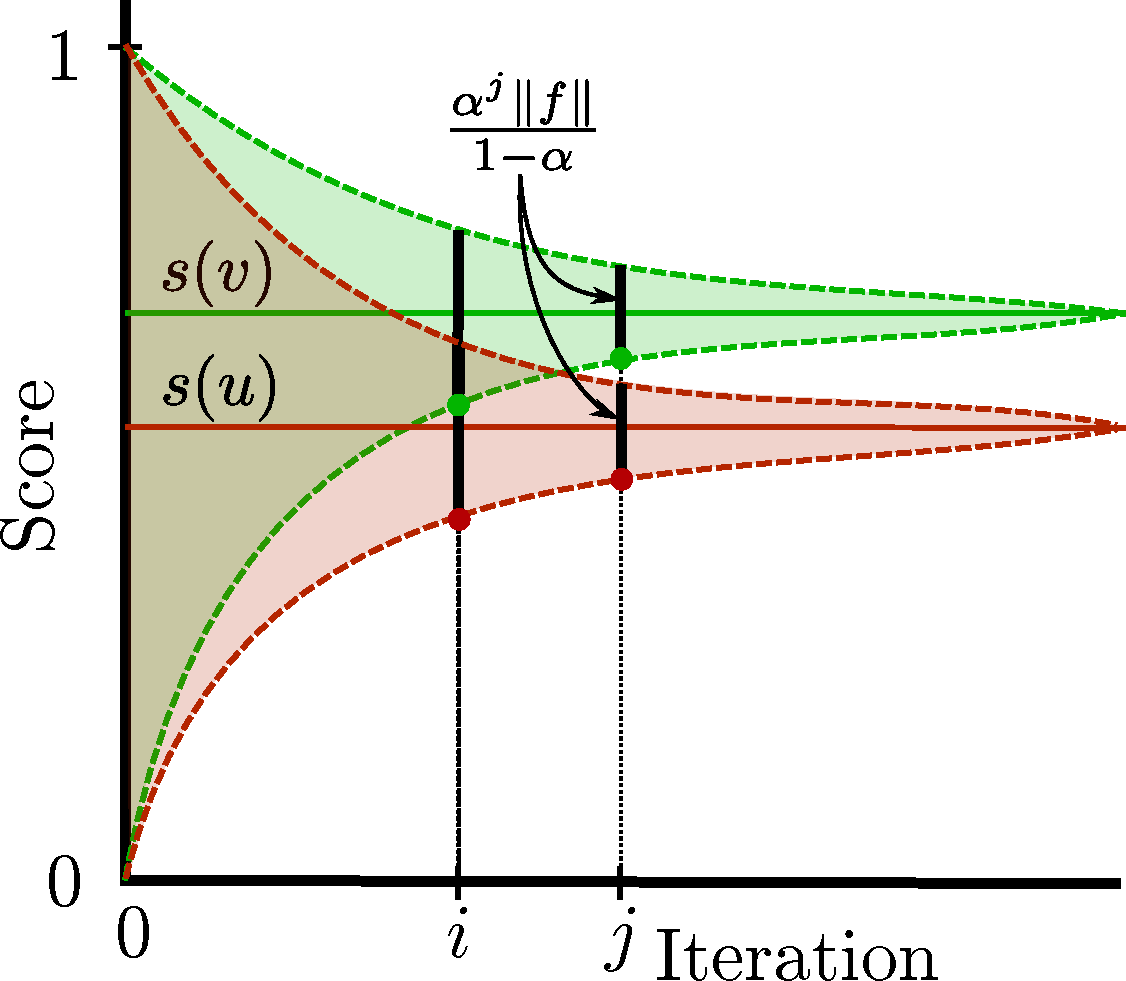
\includegraphics[width=0.4\textwidth]{figs/sink-source-squeeze-score-lb-ub-node-u-and-v-iteration-j.pdf}
    \caption{Overview of \SSS upper and lower bound comparison.}
    \label{fig:sinksource-squeeze-ub-lb}
\end{figure}

\subsubsection{\SSS proof}
TODO. See \cref{fig:sinksource-squeeze-ub-lb} for an example of the lower and upper bounds for two nodes at each iteration.

%\subsection{Lower Bound}
\par{Lower Bound}
%Each node always either increases or stays the same after each iteration. 
\begin{lemma}
\murali{State the lemma here.}
\end{lemma}

%\begin{proof}

From \cref{eq:sinksource-matrix-iteration} we have that $\vec{s}$ contains the final prediction scores for each node. We can efficiently approximate $\vec{s}$ by repeatedly iterating over \cref{eq:sinksource-matrix-iteration}, where at a given iteration $i$, 
\begin{equation}
%\label{eq:sinksource-matrix-iteration}
    \vec{s}^{(i+1)} = P\vec{s}^{(i)} + \vec{f}
\end{equation}

Below we first prove that each iteration produces a tighter lower bound vector (i.e., $\vec{s}^{(i+1)}$ closer to $\vec{s}$), and second, $\vec{s}^{(i)}$ finally converges to $\vec{s}$. 
We use the notation $\mathbf{x} \prec \mathbf{y}$ to signify that $\forall_i, x(i) \leq y(i)$.

(1) $\svec{0} = 0$, $\su{1} = f(u)$. Clearly $\svec{0} \prec \svec{1}$. Further, if $\svec{i-1} \prec \svec{i}$, then $\forall(u)$:

\begin{equation}
\su{i+1} - \su{i} = \alpha \sum\limits_{v\in{}N_u} p_{uv}\big[ \su{i} - \su{i-1}\big] \ge 0
\end{equation}

(2) Solving for \cref{eq:sinksource-matrix-iteration} gives us $\vec{s} = (I - \alpha{}P)^{-1}\vec{f}$. 
%Because $\lim_{i\to\infty}(\alpha{}P)^{i} = 0$, $(I - \alpha{}P)^{-1} = I + \alpha{}P + \alpha{}^2P^2 + \ldots \alpha{}^{\infty}P^{\infty} = \sum\limits_{j=0}^{\infty}(\alpha{}P)^j$ which was first shown in XX.
Because $\lim_{i\to\infty}(\alpha{}P)^{i} = 0$, $(I - \alpha{}P)^{-1} = \sum\limits_{j=0}^{\infty}(\alpha{}P)^j$ which was first shown in XX. \jeff{Why is this true? The limit to infinity doesn't seem to imply the second half.} Therefore we have that after every iteration, $\vec{s}^{i}$ is getting closer to $\vec{s}$.

\begin{equation}
\vec{s}^{(i)} \ = \ \sum\limits_{j=0}^{i}(\alpha{}P)^j \vec{f} \ \le \ \sum\limits_{j=0}^{\infty}(\alpha{}P)^j \vec{f} = \vec{s}
\end{equation}

Suppose $\svec{i} \prec \mathbf{s}$, then 
\begin{equation}
\su{i+1} \ \le \ \alpha \sum\limits_{v \in{} N_u} p_{uv}s(v) + f(u) \ = \ s(u)
\end{equation}
%\end{proof}

\par{Upper Bound}
\murali{Add an observation that states that $\|Ps\| \leq \|P\| \|s\|$.}

\begin{lemma}
For every node $u \in V$ and for every $i\geq 1$, $s(u) \ \le \ \su{i} + \frac{\alpha^i\|\mathbf{f}\|}{(1-\alpha)}$
\end{lemma}

Here, $\|\mathbf{x}\| = \|\mathbf{x}\|_{\infty} = \max\{|x_1|, \ldots |x_n|\}$. 
In the case of a matrix, $\|A\| = \|A\|_{\infty} = \max\limits_{i}\sum\limits_{j=0}^{n}a_{ij}$. 
Note that $\|P\| = 1$.

\textit{Proof}. $\forall i > 0$, 
\begin{align}
\svec{i+1} - \svec{i} \     &=   \ \alpha{}P(\svec{i} - \svec{i-1}) \\
\|\svec{i+1} - \svec{i}\| \ &\le \ \|\alpha{}P(\svec{i} - \svec{i-1})\| \\
                          \ &\le \ \|\alpha{}P\| \cdot \|\svec{i} - \svec{i-1}\| \\
                          \ &\le \ \alpha{} \|\svec{i} - \svec{i-1}\|
\end{align}

Repeatedly applying the above inequality gives us the following. 
\begin{equation}
\|\svec{i+1} - \svec{i}\| \ \le \ \alpha^{i} \|\svec{1} - \svec{0}\| = \alpha^{i}\|\mathbf{f}\|
\end{equation}

Now we need to account for the rest of the iterations up to $\infty$. 
We're effectively asking what is the greatest amount of score this node could accumulate in the following iterations? $\forall_m > i$
\begin{align}
\|\svec{m} - \svec{i}\| \ 
&=   \ \| \sum_{j=i}^{m-1}(\svec{j+1} - \svec{j}) \| \\
&\le \ \sum_{j=i}^{m-1}\| \svec{j+1} - \svec{j} \| \\
&\le \ \sum_{j=i}^{m-1} \alpha^{j}\|\mathbf{f}\| \\
&\le \ \alpha^i\|\mathbf{f}\| \sum_{j=0}^{m-i-1} \alpha^{j} \\
&\le \ \alpha^i\|\mathbf{f}\| \Big( \frac{1 - \alpha^{m-i}}{1 - \alpha} \Big) \\
\intertext{As $m\to\infty$, we have} 
\|\svec{m} - \svec{i}\| \ &\le \frac{\alpha^i\|\mathbf{f}\|}{(1-\alpha)}
\end{align}

\murali{The last statement is not enough. We have to prove that as $m \to\infty$, $\svec{m} \to \svec{}$.}

\murali{We also need to show that the upper bound improves as we change $i$ to $i+1$, i.e., $\su{i} + \frac{\alpha^i\|\mathbf{f}\|}{(1-\alpha)} \geq \su{i+1} + \frac{\alpha^{i+1}\|\mathbf{f}\|}{(1-\alpha)}$. In other words $\su{i+1} - \su{i} \leq \frac{(\alpha^i - \alpha^{i-1})\|\mathbf{f}\|}{1-\alpha} = \alpha^i \|\mathbf{f}\|$, which is true. }

There may be rare cases where a group of nodes have the same upper and lower bound, yet whose relative ordering with all other nodes is fixed. In these cases, we simply give them the same ranking as we have no way to distinguish how to order them in relation to each other. 

\subsection{Proof for $\alpha$}
\subsection{Proof for hierarchy consistent predictions}

A potential problem for methods which make term-based predictions is that they may not be consistent with parent-child relationships in the hierarchy. For example, if a GO term $t_i$ is a child of $t_j$, then if a method predicts a gene $g$ to be annotated with $t_i$ yet not to $t_j$, it would be inconsistent with the ontology. 
%in order to be consistent with the hierarchy, it must also predict $g$ to be annotated with $t_2$. 
In this section we provide a proof for \sinksource and \genemania that all predictions are hierarchically consistent.
%Specifically 

Let $s_i(u,k)$ be the score of node $u$ after $k$ iterations of \sinksource for a given term $t_i$. 
In order to give hierarchically consistent predictions, $s_i(u,k)$ must be $\leq s_j(u,k)$ at each iteration $k$, meaning for a given parent-child term pair, the prediction score of a gene for the parent term must always be equal to or greater than the score for the child term.
%meaning the prediction score of $u$ after $k$ iterations for $t_2$ must be $\leq$ the score of $u$ after $k$ iterations for $t_2$. \jeff{don't repeat, summarize here}

\begin{theorem}
For every parent $t_j$ and child $t_i$ term pair, node $u \in V$, and iteration $k$, $s_i(u,k) \leq s_j(u,k)$
\end{theorem}

First, we show the relationships between positive and negative examples for $t_i$ and $t_j$, then use them to prove the scores only either increase or stay the same when for a given node as we make predictions for terms higher in the hierarchy. 
According to our definition of negative examples (see \cref{sec:pos-neg-unk-examples}), all genes directly annotated with a term other than $t_i$ its ancestors will be considered a negative example for $t_i$. 
Let $V^+(t_i)$, $V^-(t_i)$, and $V^0(t_i)$ be the sets of positive, negative and unknown example for term $t_i$.  %\jeff{by def.} 
All positive, negative and unknown examples for $t_i$ and $t_j$ would be the same, except in the following two observations.
%The differences of positive, negative, and unknown examples from $t_i$ to $t_j$ are encompassed in the following three observations.
\begin{enumerate}[i.]
    \item $V^+(t_i) \subseteq V^+(t_j)$ and $V^-(t_i) \supseteq V^-(t_j)$. Genes directly annotated to siblings of $t_i$ and their descendants, would be positive examples for $t_2$, yet negative examples for $t_i$.
    %\item $V^+(t_i) \subseteq V^+(t_j)$. Genes directly annotated to siblings of $t_i$ and their descendants, would be positive examples for $t_2$, yet negative examples for $t_i$
    %\item $V^-(t_i) \supseteq V^-(t_j)$. Same reasoning as above.
    \item $V^0(t_i) \subseteq V^0(t_j)$. Genes annotated directly to $t_j$ would be positive examples for $t_j$ and unknown examples for $t_i$.
\end{enumerate}
%We observe that , $V^-(t_i) \supseteq V^-(t_j)$, and $V^0(t_i) \subseteq V^0(t_j)$ as  would be genes which are directly annotated to $t_j$ and its descendent terms, excluding $t_i$ and its descendants. %which would be positive examples for both $t_1$ and $t_2$. 
%Let $D(t_i)$ include $t_i$ and its descendants in a given hierarchy.
%sibling terms of $t_1$, or other 
%Genes directly annotated to descendants of $t_j$, excluding $t_1$ and its descendants, would be positive examples for $t_2$, yet negative examples for $t_1$. 
%$U(t_2) = U(t_1) - P(t_2)$. 
Below we prove $s_1(u,k) \leq s_2(u,k)$ at each iteration $k$ by induction.

\paragraph{\sinksource.}
Base case: $s_1(u,1) \leq s_2(u,1)$.
\begin{align}
    s_i(u,1) &= \alpha \sum_{\mathclap{v \in N^0_i(u)}} p_{uv}s_i(v,0)  + f_i(u) = 0 + f_i(u) \\
    s_j(u,1) &= \alpha \sum_{\mathclap{v \in N^0_j(u)}} p_{uv}s_j(v,0)  + f_j(u) = 0 + f_j(u)
\end{align}
where $N^0_i(u)$ is the neighbors of $u$ in $V^0$ for $t_i$.
%\shortintertext{Because $P(t_1) \subseteq P(t_2)$ and $N(t_1) \supseteq N(t_2)$ the 
Because of the observation that $V^+(t_i) \subseteq V^+(t_j)$ and $V^-(t_i) \supseteq V^-(t_j)$, $f_i(u)$ would have less positive neighbors and more negative neighbors than $f_j(u)$, meaning
\begin{align}
      f_i(u) &\leq f_j(u) \label{eq:fi_leq_fj}%\\
%\shortintertext{thus proving}
%    s_1(u,1) &\leq s_2(u,1)
%    \alpha\sum_{\mathclap{v \in N^{+}_{1}(u)}} P_{uv}(1) &\leq \alpha\sum_{\mathclap{v \in N^{+}_{2}(u)}} P_{uv}(1)
\end{align}
%where $f_i(u) = \alpha \sum_{v \in N^{+}_{i}(u)} P_{uv}(1)$ is the amount of fixed score coming from neighbors of $u$ in $V^+$ for term $t_i$. Negative examples are fixed at $0$ and therefore do not contribute to the score. \jeff{move this above}
%Because $V^+(t_1) \subseteq V^+(t_2)$ and $V^-(t_1) \supseteq V^-(t_2)$, meaning $t_2$ has more positive and less negative examples than $t_1$, \cref{eq:f1_leq_f2} holds.
Suppose that $s_i(u,k-1) \leq s_j(u,k-1)$.
By the inductive hypothesis, we show $s_i(u,k) \leq s_j(u,k)$ as follows
\begin{align}
    s_i(u,k) &= \alpha \sum_{\mathclap{v \in N^0_i(u)}} p_{uv}s_i(v,k-1) + f_i(u)  \\
          &\leq \alpha \sum_{\mathclap{v \in N^0_i(u)}} p_{uv}s_i(v,k-1) + f_j(u) \text{, \cref{eq:fi_leq_fj}} \\
          &\leq \alpha \sum_{\mathclap{v \in N^0_j(u)}} p_{uv}s_j(v,k-1) + f_j(u) \text{, by the inductive hypothesis} \\
             &= s_j(u,k)
\end{align}

thus completing the proof.
%The above reasoning holds true for all ancestors of $t_i$, thus ensuring that for genes, all predictions are hierarchically consistent.


\subsection{Datasets}
\label{sec:datasets}

\subsubsection{Sequence Similarity Network}
\label{sec:ssn}
We created a network based upon sequence similarity of the putative proteomes of 19 clinically-relevant pathogenic bacteria.
We downloaded sequences and GO annotations from UniProt~\cite{uniprot-consortium-uniprot-nar-2017}.
In instances where multiple UniProt reference strains were available for a pathogen, we chose the reference proteome with the largest number of GO annotations.
We performed an all-vs-all BLASTP and processed the results by 
%removing \evals $\geq$ 0.1,
%(ii) deleting matches where the length of the sequences differed by $>$ 20\%, % effusion has a better description for this processing step
retaining the weaker score for all reciprocated matches, removing self-comparisons, and using the absolute value of the base-10 logarithm of the \eval as the edge weight. 
For edges where the \eval was 0, we assigned a score of 180 which is the -log$_{10}$ of the smallest non-zero \eval observed (rounded).
For networks where we used an \eval cutoff $> 1$, we added log$_{10}$ of the cutoff to the edge scores to ensure all edges had a positive score.
We tested various \eval cutoffs from \e{-25} to 50 (see Table \ref{tab:net-sizes} for the number of nodes and edges).
%The resulting network (referred to as \SSN) contained 60K proteins connected by 2.5M edges.

\subsubsection{STRING Networks}
\label{sec:string}
We integrated species-specific STRING functional association networks for 14 of the 19 bacterial species where ID mapping from UniProt was available (STRING v10.5, downloaded on 2017.09.18)~\cite{szklarczyk-mering-string-v10.5-nar-2017}.
% We recognize that using a more sophisticated method such as that used by INGA of mapping using BLAST would increase our coverage, however, the ID mapping worked well enough for our evaluations here.
STRING assigns edge weights based on evidence of association including physical binding, gene expression, orthology mapping and more. 
Specifically, we utilized six STRING networks: neighborhood, fusion, cooccurence, coexpression, experimental, and database.
% move this point to discussion or results
We found including all available networks did not improve the quality of results above the six core networks (results not shown).
%We chose not to include the networks with evidence transferred based on orthology to ensure that when performing an evaluation for a given species, we did not transfer evidence from 
%Combining those 50K nodes and 2.4M associations with the SeqSim network yielded a network (referred to as Integrated) with 70K nodes and 5M edges.
We also tested various STRING cutoffs including 150, 400 and 700 (low, medium and high stringency) cutoffs (see Table \ref{tab:net-sizes} for network sizes). 
%\murali{Move to supplement; you can refer to this table in the main text.}



\subsubsection{Gene Ontology Annotations}
\label{sec:goa}
We obtained GO~\cite{gene-ontology-consortium-go-expansion-nar-2017} annotations for these bacteria from the UniProt-GOA database (``goa\_uniprot\_all.gaf.gz'' Downloaded on 2017.09.18).
% ftp://ftp.ebi.ac.uk/pub/databases/GO/goa/UNIPROT/goa_uniprot_all.gaf.gz
%We considered two subsets of annotations: (a) EXP: only based on experimental evidence codes and (b) non-IEA: EXP codes as well as codes based on curator verified sequence similarity annotations. A total of 154 molecular function (MF) and 453 biological process (BP) GO terms were annotated to at least 100 proteins with a non-IEA evidence code. 13K proteins had at least 1 non-IEA annotation, and 6K had at least 1 EXP annotation. For each GO term, we treated every gene that was not annotated to any ancestor or to any descendant term as a negative example.
%
% evidence codes
We considered three sets of evidence codes: (i) Experimental as well as those used in CAFA (EXPC): EXP, IDA, IPI, IMP, IGI, IEP, TAS, IC; (ii) Computational Analysis (COMP): ISS, ISO, ISA, ISM, IGC, IBA, IBD, IKR, IRD, RCA; and (iii) Electronic Analysis (ELEC): IEA.
A total of 319 biological process (BP) and 117 molecular function (MF) GO terms were annotated to at least 50 proteins with an EXPC evidence code.
% We recognize there is a potential circularity issue where the 

%\subsubsection{Selecting Bacterial Species}
%As a proof-of-concept, we selected 19 clinically relevant bacteria. 
%%We also sought to scale-up to include many more bacterial species. 
%To scale-up to include many more organisms, we simply selected the top 200 bacterial species with the most EXPC or COMP annotations which ranged from six to 16,685 (\textit{Gluconobacter oxydans} and \textit{Escheria coli} respectively).

\subsubsection{Positive, Negative, and Unknown Examples}
\label{sec:pos-neg-unk-examples}
We say that $g$ is \emph{directly} annotated to $t$ if this annotation appears in the annotations (GAF) file. For a given GO term $t$, we defined a gene $g$ as 
\begin{enumerate}[(a)]
    \item a \emph{positive example} if $g$ was directly annotated to $t$ or to a descendant of $t$ in the GO DAG, 
    \item a \emph{negative example} if $g$ was not directly annotated to $t$ or to an ancestor or descendant of $t$ in the GO DAG, but also had at least one other annotation, and 
    \item an \emph{unknown example} otherwise.
\end{enumerate}
This approach is commonly used in the literature~\cite{mostafavi-morris-genemania-gb-2008}.
%  and a given set of positive evidence codes $EC$  % with an evidence code in $EC$
In several analyses, we restricted our attention to a specific set of evidence codes, e.g., experimental ones. In such a situation, we discarded all direct annotations with other evidence codes before computing the different sets of examples.
%For example, if we used EXPC annotations to define positive examples, we also used EXPC annotations to define negative examples.
%Additionally, if $g$ was assigned as a negative example for $t$ but has an electronic annotation  (i.e., IEA), we removed it as a negative example for $t$.
In addition, if a gene $g$ satisfied the conditions to be a negative examples for a term $t$ but also had an electronic annotation (i.e., evidence code IEA) to $t$, we considered $g$ to be an unknown example for $t$.
%Improving our selection of negative examples would improve the performance at various 

We utilized these three sets of examples in different aspects of this work: (a) for integrating multiple networks, (b) for algorithms which use negatives examples (\sinksource and \genemania), and (c) for defining false positives when evaluating. \murali{Add section numbers.}


\subsection{Network Integration}
\label{sec:network-integration}
%\jeff{probably shouldn't go under datasets}
We compared two kernel-based network integration methods.
\begin{description}
\item[1) \genemania-2008] \hfill \\
Mostafavi and Morris integrated multiple networks on a GO term-by-GO term basis using ridge regression~\cite{mostafavi-morris-genemania-gb-2008}. %Loosely, for a given GO term, the networks are given a score based on how well the edge weights match the positives vs. the negatives. The networks are then combined by taking the sum of the edge weights in each network, multiplied by its score.
Given $m$ \FLN{}s encoded as matrices $W_{1},...,W_{m}$, they combined the networks using:

\begin{equation*}
    W^{comb} = \sum\limits_{i=0}^{m} \mu_{i}W_{i}
\end{equation*}

where the network weights, $\mu = [\mu_1, \mu_2, ..., \mu_m]$, are assigned by solving a constrained linear regression problem for a specific prediction task. 
\jeff{Include the equation here}.

\item[2) SWSN] \hfill \\
%Mostafavi and Morris later improved their original method by computing optimal weights for multiple related GO terms simultaneously~\cite{mostafavi-morris-fast-integration-bioinfo-2010}.
Youngs \etal followed a similar framework where they compute an optimal weight for each network, however they extend the method to be able to compute the weights for multiple related GO terms simultaneously using specific negative examples (Simultaneous Weights with Specific Negatives, SWSN)~\cite{youngs-bonneau-better-negatives-pfp-bioinfo-2013}. 
They found that fitting the weights to all GO terms in a particular hierarchy (i.e., BP or MF) worked better than any other grouping of functions. 
We also grouped GO terms by hierarchy to compute the optimal weights for our networks.
%once for a given set of GO terms with an approach similar to the previous method in the case of individual GO terms~\cite{youngs-bonneau-better-negatives-pfp-bioinfo-2013}. While there are many ways to combine the GO terms, we only used the sets of all GO terms in a given hierarchy (BP or MF) which they found performed the best.

\end{description}
% discussion section?
% In our experiments, we found that the in
Interestingly, in our experiments we found that using the original integration method proposed by Mostafavi \etal resulted in better performance than the SWSN method for \sinksource and \genemania, especially for MF GO terms (results not shown).
For \birgrank, we were limited to the SWSN method as for a given protein, all GO term predictions (for a given hierarchy) are made simultaneously.


\subsection{Evaluation}
\label{sec:evaluation}
\subsubsection{Leave-One-Species-Out Evaluation}
We evaluated each algorithm using a leave-one-species-out validation method where we iteratively leave out the annotations of all proteins of a single species, and use the annotations of the other 18 species to make predictions for the left out species (see \fig \ref{fig:leave-one-species-out}). This evaluation is meant to test our ability to make functional predictions for the genome of a newly sequenced species where none of the proteins have any previous annotations. 

\begin{figure}[htb]
    \centering
    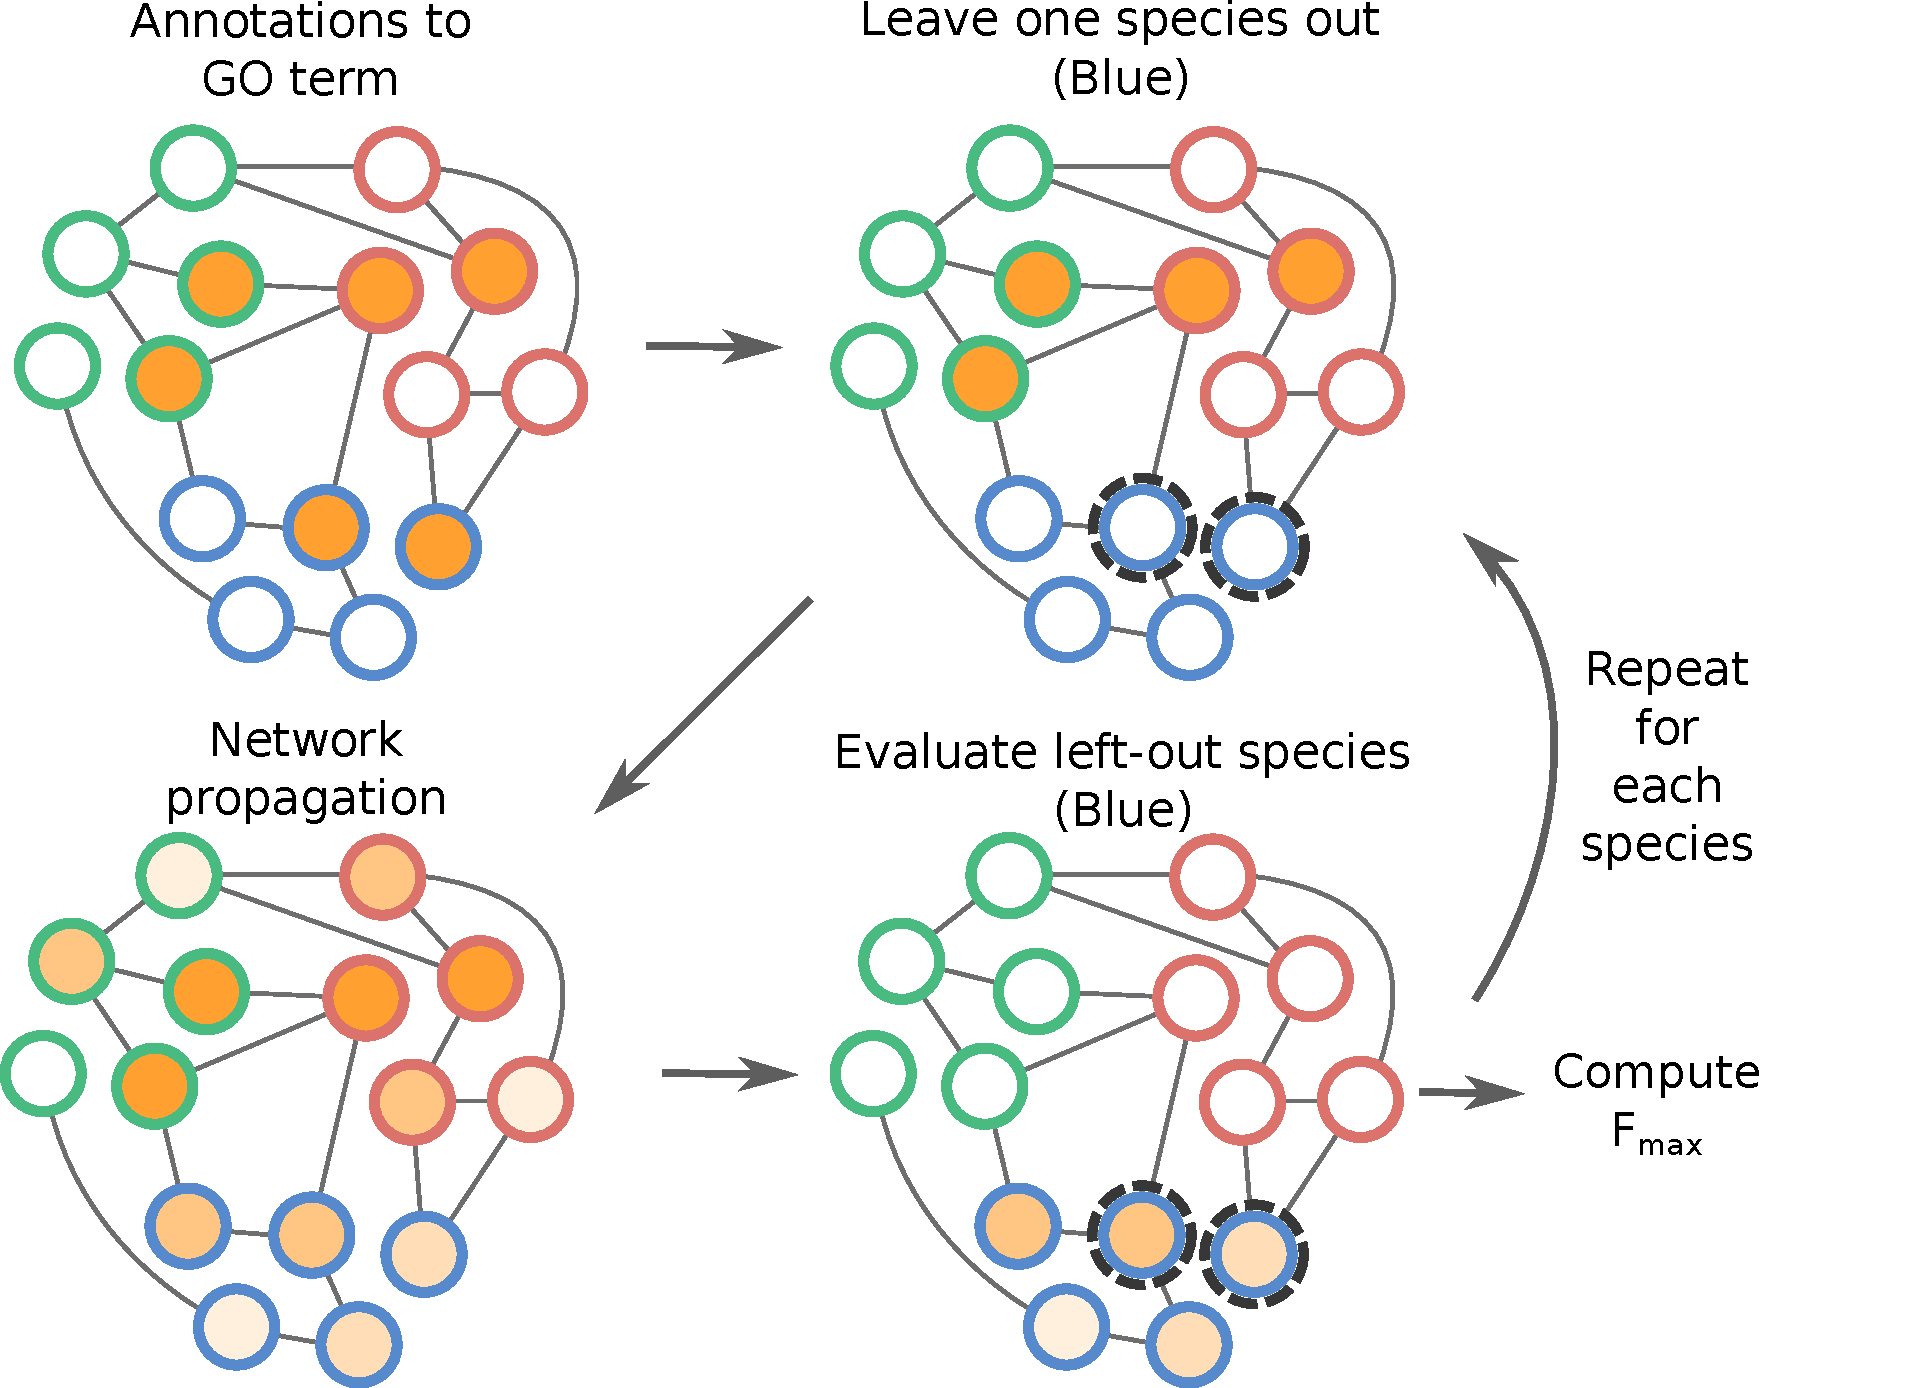
\includegraphics[width=0.5\textwidth]{figs/leave-one-species-out.pdf}
    \caption{Overview of the leave-one-species-out evaluation. The picture represents a \SSN where the border colors represent a species. The orange nodes represent proteins annotated with a given GO term (top left). All annotations are left out for a given species (top left) and evaluated how well they can be recovered (bottom right) by propagating the annotations from the known proteins to the nearby unknown proteins (bottom left). This process is repeated for all GO terms and all species.}
    \label{fig:leave-one-species-out}
\end{figure}

We chose to first evaluate using only the experimentally-based annotations. 
When evaluating predictions for a given left-out species, true positives and false positives are calculated from the positive and negative examples of that species.
%However, as only a few species have a decent amount of experimentally-based annotations, we also expanded our evaluation to include annotations with either an experimental, or computational evidence codes as defined above. 
%A total of 9 species have at least one GO term for which 10 or more proteins are annotated. 

We used the \fmax value to compare algorithms, as it is used in the critical assessment of functional annotation (CAFA) challenge. 
%\subsubsection{Temporal Holdout}
%June 2016 - September 2017